\chapter{Grundlagen der medizinischen Bildverarbeitung} \label{grundlagen}
\addthumb{Grundlagen der medizinischen Bildverarbeitung}{\huge{\textbf{\thechapter.}}}{white}{haw_rot}

\section{Bildgewinnung und bildgebende Verfahren}

\section{DICOM}
Der Name DICOM steht für \textit{Digital Imaging and COmmunication in Medicine}. Der Umgang mit diesem Standard ist essentieller Bestandteil der zu entwickelnden Software. Pianykh\cite{pianykh:dicom} beschreibt im ersten Kapitel, dass DICOM nicht nur aus Pixel und deren zugehörigen Werten besteht. Wie der Name sagt, ist auch die Kommunikation fest im Standard verankert. Damit ist die Übertragung der Daten von medizinischen Geräten(Modalitäten) zum zentralen Speicher und deren Verteilung gemeint. Des weiteren spielt die dauerhafte Speicherung der digitalen Aufnahmen eine große Rolle. Daher wird im gleichen Zug mit DICOM immer ein PACS genannt. Die Abkürzung PACS bedeutet \textit{Picture Archiving and Communication System} und besteht sowohl aus Hardware (Server, Speicherung) als auch Software(Verteilung und Kommunikation).\\
Abbildung \ref{communication} illustriert das Zusammenspiel des DICOM-Standards und dem zentralen Datenspeicher. Zuerst wird mittels der Modalitäten(z.B. mit dem Computertomographen oder einem Ultraschallgerät) die digitale Aufnahme erzeugt. Danach wird das Bild vom Gerät an das PACS gesendet. Hier werden die Aufnahmen und Patientendetails in die Datenbank und den Speicher abgelegt. Wird eine Aufnahme benötigt können Clients Anfragen mit beispielsweise dem Patientennamen stellen und erhalten die zugehörige Serie mit der digitalen Aufnahme.

\begin{figure}[htbp]
  \vspace{0.5cm}
  \centering
  \fbox{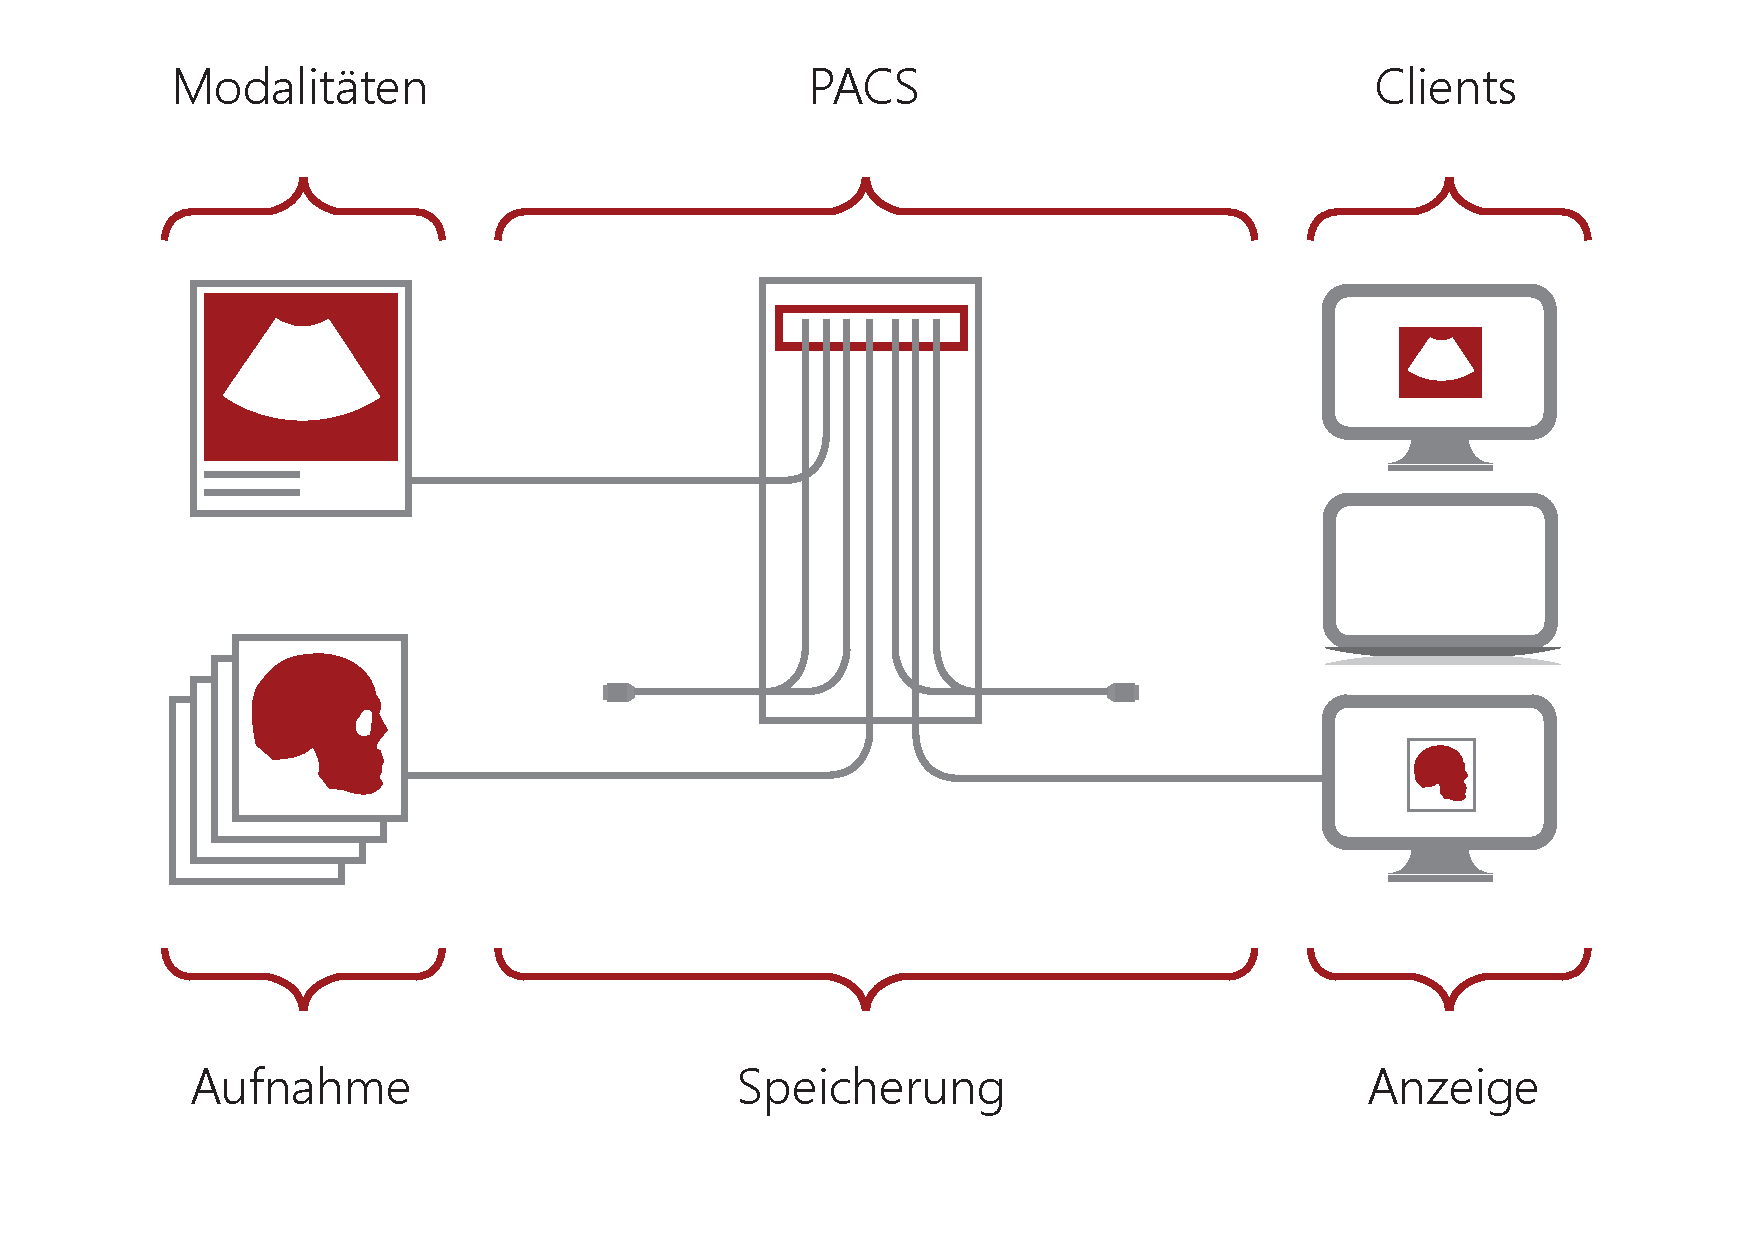
\includegraphics[angle=0,width=12cm]{./img/communication_neu.pdf}}
  \caption{Kommunikationsprozess von Aufnahme zur Verarbeitung}
  \floatfoot{Vorlage für diese Darstellung ist die Grafik in \cite[Fig. 1]{pianykh:dicom}}
  \label{communication}
  \vspace{0.5cm}
\end{figure}

DICOM\footnote{Unter ftp://medical.nema.org/medical/dicom/ lässt sich der aktuelle Standard abrufen. Die Kapitel befinden sich im Ordner zum jeweiligen Jahr der Veröffentlichung. Aktuell sind die Dokumente von 2011.} ist daher nicht nur ein einzelner Standard, sondern verknüpft die standardisierte 
\begin{itemize}
\item Kommunikation,
\item Erzeugung der Bilddaten,
\item und Speicherung.
\end{itemize}
Im Rahmen dieser Abschlussarbeit liegt der Fokus auf den Bilddaten, daher wird auf die Kommunikation- und Speicheraspekte nicht im Detail eingegangen.

\subsection{Die Dicom Information Object Definitionen} \label{grundlagen:iod}
Bevor die Pixeldaten genauer betrachtet werden können, muss der prinzipielle Aufbau der Dicomobjekte beschrieben werden. Teil 3 des Standards\cite[A.1.2]{dicom:iod} zeigt den relationalen Aufbau der Dicomobjekte. Vereinfacht können die elementaren Informationsobjekte in drei Teile aufgeteilt werden.

\begin{itemize}
	\item \textbf{Patient}\\
	Der Patient steht in der Hierarchie an oberster Stelle und ist die Grundlage für eine oder mehrere Studien(Study).
	\item	\textbf{Study}\\
	Study symbolisiert eine medizinische Studie. Eine Studie ist eine Sammlung von mehreren Serien, die von Modalitäten wie CT und MR aufgezeichnet werden. Eine Studie ist exakt einem Patient zugeordnet.
	\item \textbf{Series}\\
	Eine Serie ist ein Folge von Bildern, die von einer Modalität erzeugt wird. Die Aufnahmen eines CT werden einer Serie zugeordnet. Jede Serie gehört zu nur einer Studie.
	\item \textbf{Image, Real World Values}\\
	Auf der unteren Hierarchiestufe stehen Objekte wie Bilddaten oder die Lage des Patienten im Raum während der Aufnahme. Ein Bild wird genau einer Serie zugeordnet.
\end{itemize}

Aus diesen vier elementaren Objekten ergibt sich folgende Informationsstruktur für Dicomobjekte, die in Abbildung \ref{ermodel} als Entity-Relationship-Modell\footnote{Ein ER-Modell beschreibt die Beziehungen der Elemente zueinander. Dieser Diagrammtyp wird unter Anderem häufig beim Entwickeln der Struktur einer relationalen Datenbank verwendet} verdeutlicht wird.

\begin{figure}[htbp]
  \vspace{0.5cm}
  \centering
  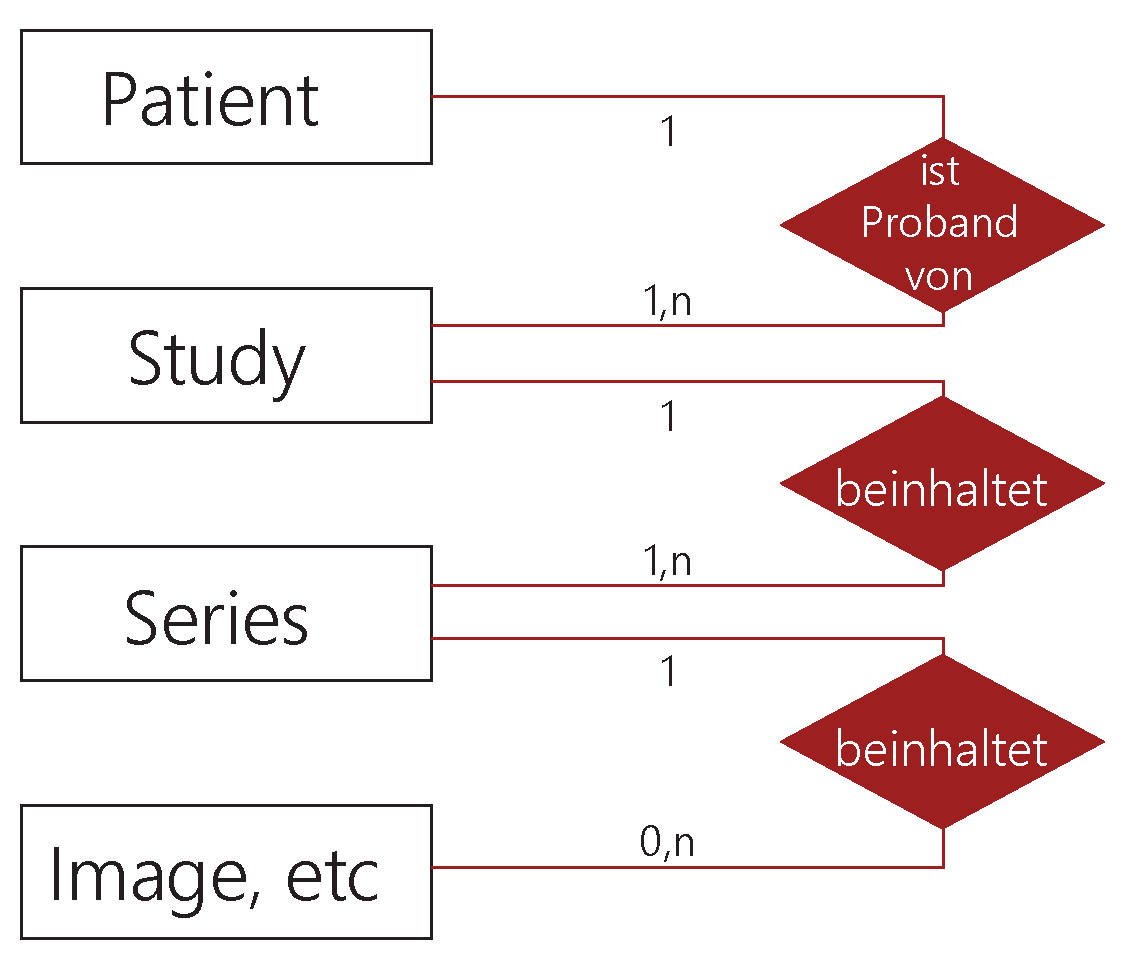
\includegraphics[angle=0,width=8cm]{./img/ermodel.pdf}
  \floatfoot{Vorlage für diese Darstellung ist die Grafik in \cite[A.1.2]{dicom:iod}}
  \caption{Vereinfachte Darstellung der Informationsobjekthierarchie von Dicomelementen}
  \label{ermodel}
  \vspace{0.5cm}
\end{figure}

Der DICOM-Viewer OsiriX bietet auf der Herstellerseite\footnote{http://www.osirix-viewer.com/datasets/} die Möglichkeit Testdaten zu beziehen. Betrachtet man die Repräsentation der Daten auf der Festplatte hält sich die Ordnerstruktur an obiges ER-Modell.\\
Abbildung \ref{filesystemrep} zeigt eine schmatische Darstellung der Dateien. Die Beispieldaten von OsiriX bestehen aus einem Patient names \glqq Brebix\grqq, dem eine Studie sowie zwei Serien à 100 Aufnahmen zugeordnet werden.

\tikzstyle{every node}=[draw=black,thick,anchor=west]
%\tikzstyle{selected}=[draw=red,fill=red!30]
\tikzstyle{optional}=[dashed,fill=gray!50]
\begin{figure}[htbp]
\centering
\caption{Repräsentation der Information Objekte im Dateisystem}
\label{filesystemrep}
\begin{tikzpicture}[%
  grow via three points={one child at (0.5,-0.7) and
  two children at (0.5,-0.7) and (0.5,-1.4)},
  edge from parent path={(\tikzparentnode.south) |- (\tikzchildnode.west)}]
  \node {Dicom Ordner}
    child [missing] {}
    child { node {BREBIX - Patient}
    	child [missing] {}
    	child { node{CT10 ponction foie - Studie}
    		child [missing] {}
    		child { node {DEF FOIE ART. - 107198 - Serie}
    			child{node[optional]{IM-0001-0001.dcm}}
    			child{node[optional]{...}}
    			child{node[optional]{IM-0001-0100.dcm}}
    		}
    		child [missing] {}				
    		child [missing] {}				
    		child [missing] {}
    		child [missing] {}
    		child { node {DEF. VEINEUX - 107205 - Serie}
    		    child{node[optional]{IM-0001-0001.dcm}}
    		    child{node[optional]{...}}
    		    child{node[optional]{IM-0001-0100.dcm}}
    		}
    		child [missing] {}
    	}
    };		
\end{tikzpicture}
\end{figure}

Bei näherem Hinsehen fällt auf, dass die Dateinamen beider Serien des Patienten identisch sind. Eine korrekte Zuordnung von DICOM-Dateien zur Serie ist daher nicht immer garantiert. Unabhängig von einer Repräsentation im Dateisystem oder Pfadangaben in der Datenbank eines PACS ist das Vertrauen auf Dateipfade unsicher, da über eine einfache Dateimanipulation die Zuordnung nicht mehr hergestellt werden kann.\\
Um eine zuverlässige Verknüpfung zu gewährleisten besitzt jeder Patient\footnote{Die Identifikationsnummern von Patienten sind meist nur innerhalb einer Institution oder Krankenhauses einzigartig, da diese manuell vergeben werden können\cite[5.6.2]{pianykh:dicom}.}, jede Studie und Serie eine Eindeutige Identifikationsnummer. Diese Art der Informationen wird in den einzelnen Dateien mit Hilfe von Einträgen aus dem DICOM Data Dictionary\cite{dicom:dd} hinterlegt. Die DICOM-Dateien beschreibt Pianykh \cite[S. 47]{pianykh:dicom}
als eine Kopie im Speicher vom tatsächlichen DICOM-Objekt.

\subsection{Der Transfer vom Patienten zu digitalen Dicomobjekten} \label{grundlagen:dicomObjects}
Wie der Name bereits andeutet ist das DICOM Data Dictionary vergleichbar mit einem Wörterbuch. Es enthält alle gültigen Elemente, die zur Beschreibung eines DICOM-Objekts verwendet werden können. Zusätzlich zu dem aus dem Standard bekannten Vokabular können Hersteller medizinischer Geräte ein eigenes Dictionary hinzufügen. Die proprietären Elemente können allerdings nicht standardisiert verarbeitet werden(vgl. \cite[S.45]{pianykh:dicom}, da Software die diese Objekte verarbeitet nichts von der Existenz dieser Elemente weiß).\\
Mit Hilfe des Wörterbuchs und den ca. 2000 enthaltenen Daten können nun Aussagen des wirklichen Lebens (vorausgesetzt die Aussage ist mit einem Element aus dem Wörterbuch darstellbar) ins Digital übersetzt werden.\\
Tabelle \ref{table:patientname} zeigt das DICOM-Element für den Namen des Patienten aus dem Data Dictionary\cite[S. 14]{dicom:dd}.

\begin{table}
    \begin{tabularx}{\textwidth}{|X|X|X|X|X|}
    \toprule
    \hline
    \textbf{Tag}         & \textbf{Tagname}     & \textbf{VR} & \textbf{Wert}     	& \textbf{VM} \\ \hline
    (0010,0010) 		 & PatientName 			& PN 		  & John\^{}Doe 		& 1  \\  \hline
    \bottomrule
    \end{tabularx}
    \caption {Repräsentation des Patientennamen als DICOM-Element}
    \label{table:patientname}
\end{table}

Betrachtet man den folgenden Satz(vgl. \cite[S.46]{pianykh:dicom}), kann dieser in ein DICOM-Object, wie es Tabelle \ref*{table:translation} darstellt, übersetzt werden:
\begin{center}
\textit{\glqq John Doe, männlich, geboren am 01. Januar 1970\grqq}
\end{center}

Aus den Beispielen von Tabelle \ref{table:patientname} und \ref{table:translation} lässt sich erkennen, dass ein DICOM-Element nochmals in atomare Teile aufgespalten werden kann. Folglich besteht ein Datenelement aus einem beschreibenden \textit{Tag}, einer \textit{VR(Value Representation)}, einem Wert und der \textit{VR (Value Multiplicity)}. Das Element selbst nimmt eine von drei Darstellungsmöglichkeiten ein. Abhängig von der Transfersytax\footnote{Unter der Transfersystax verstehn man eine Menge an Kodierungsvorschriften von DICOM-Objekten\cite[S.63 Section 10]{dicom:structure}. Zu diesen Vorschriften gehört zum Beispiel die Reihenfolge der Bytes im DICOM-Element oder die Komprimierung der Bilddaten} des DICOM-Objekts ist der VR-Teil optional. Die weiteren beiden Darstellungen unterscheiden sich in der Kodierung der benötigten Länge des Werts \cite[7.1]{dicom:structure}.  Anhang \ref{appendix:speicher} auf Seite \pageref{appendix:speicher} zeigt wie Datenelemente im Speicher abgelegt werden und wie viel Speicherplatz pro Element reserviert werden muss.

\begin{table}
    \begin{tabularx}{\textwidth}{|p{4cm}|p{4cm}|X|X|X|}
    \toprule
    \hline
    \textbf{Tag\newline \small{(Gruppe, Element)}}         & \textbf{Tagname}     & \textbf{VR} & \textbf{Wert}     	& \textbf{VM} \\ \hline
    (0010,0010) 		 & PatientName 			& PN 		  & John\^{}Doe 		& 1  \\ \hline
    (0010,0030) 		 & PatientBirthDate		& DA 		  & 19700101	 		& 1  \\ \hline
    (0010,0040)			 & PatientSex 			& CS 		  & M			 		& 1  \\ \hline
    (0010,1010) 		 & PatientAge 			& AS 		  & 44			 		& 1  \\ \hline
    \bottomrule
    \end{tabularx}
    \caption {Das erzeugte DICOM-Objekt mit den Elementen zu Patientenname, Geburtsdatum, Geschlecht und Alter}
    \label{table:translation}
\end{table}


%ftp://medical.nema.org/medical/dicom/2011/11\_05pu.pdf Seite 39